\chapter{Compact Muon Solenoid Experiment
\label{ch:cmsexperiment}}
\setcounter{section}{-1}

The Compact Muon Solenoid experiment is one of two general-purpose detectors at the LHC. It is located about 100\unit{m} underground at Point 5 of the LHC ring, near Cessy, France. The detector is cylindrically shaped, with total length 22\unit{m}, diameter 15\unit{m}, and weight 14000\unit{tons}. Figure \ref{fig:cms-overall} shows the overall layout of the detector.

\begin{figure}[hbt]
\begin{center}
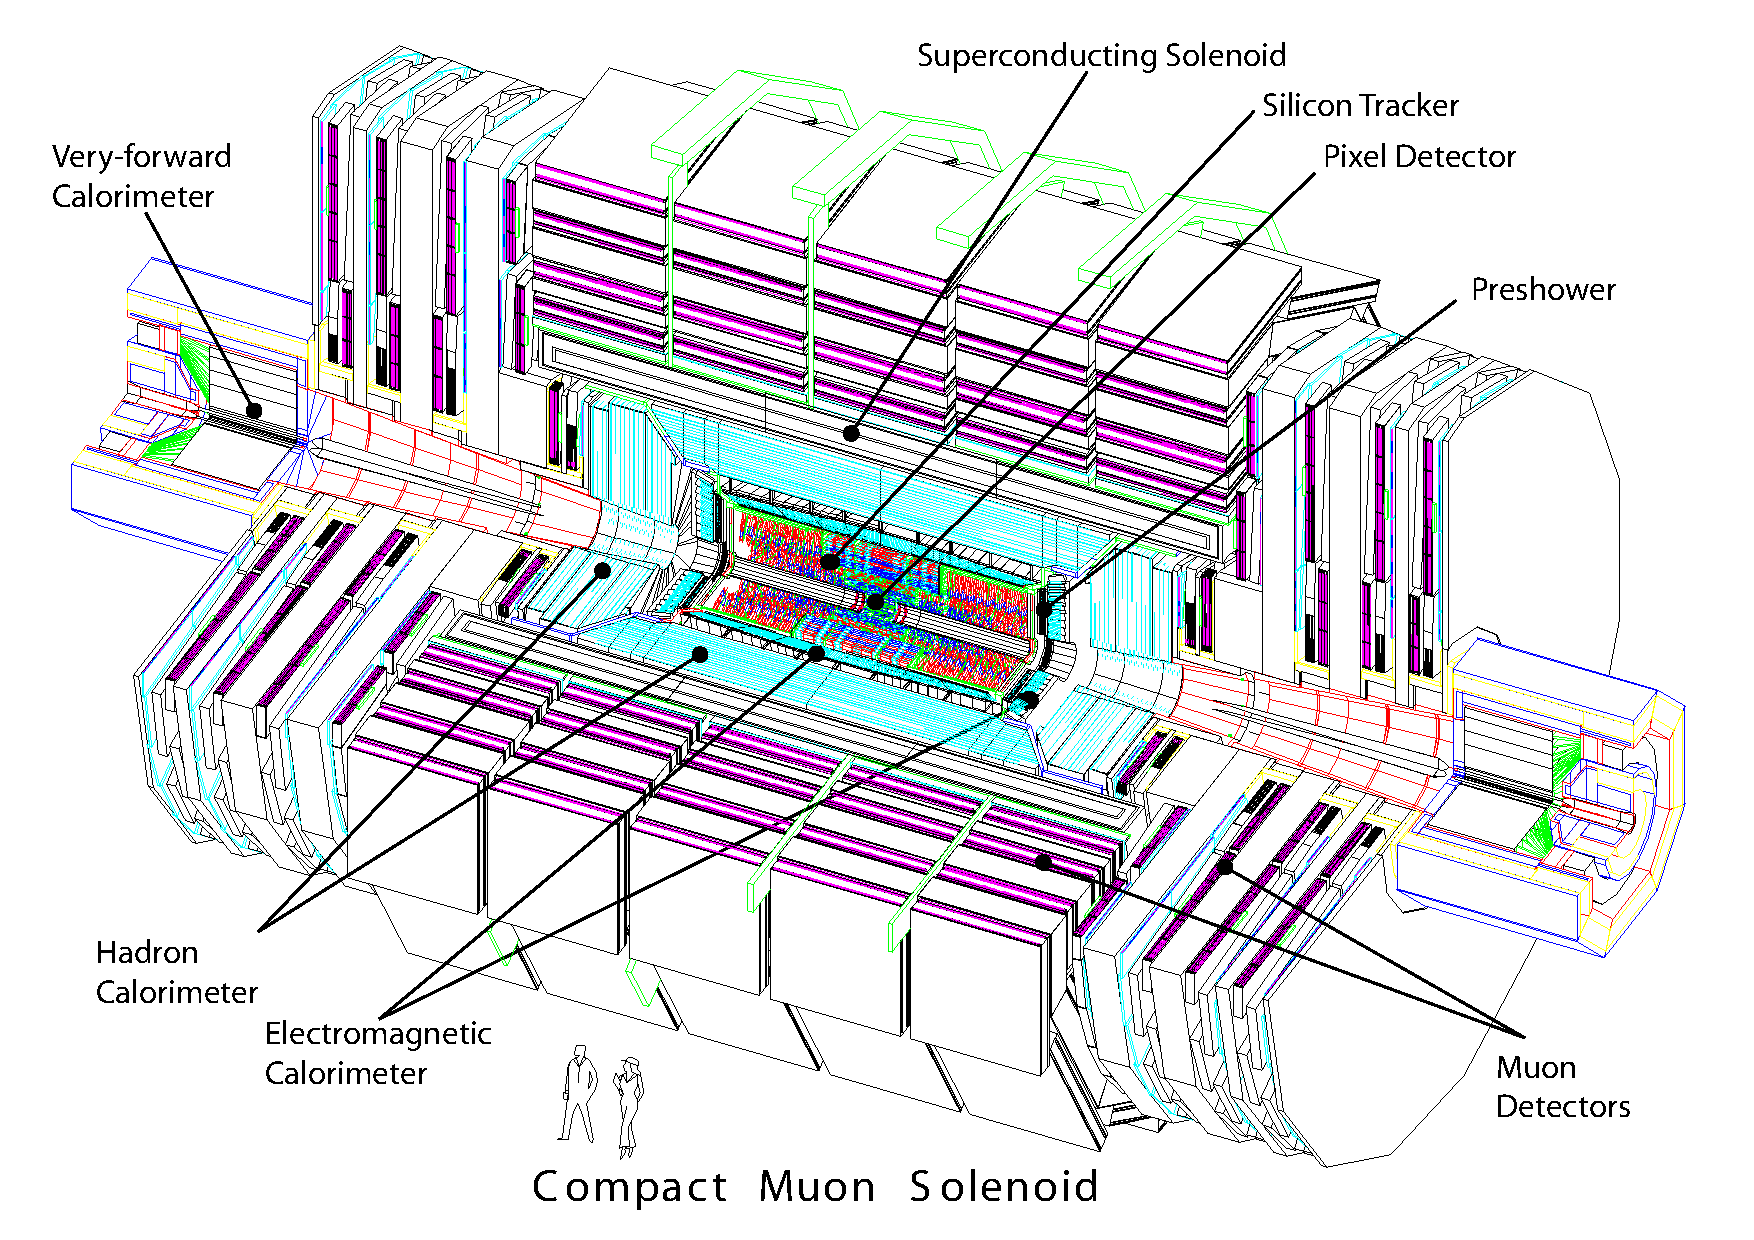
\includegraphics[width=0.95\textwidth]{figures/cms_complete_labelled.pdf}
\caption{The layout of the CMS detector, with the subdetectors labeled and two humans shown for a height reference.}
\label{fig:cms-overall}
\end{center}
\end{figure}

The center of the detector, the interaction point (IP), is used as the origin of the right-handed coordinate system that describes locations and directions within the detector. The $z$-axis is assigned to the direction of the LHC beam line, pointing anti-clockwise in the direction of Beam 2. The polar angle $\theta$ is defined as the angle away from the positive $z$-axis. This angle is often transformed into pseudorapidity, defined as $\eta = -\text{ln}[\text{tan}(\theta/2)]$, which has several desirable properties. It is independent of the particle mass and energy, and it is approximately equal to the rapidity for relativistic particles. Differences in pseudorapidity are Lorentz invariant for boosts in the $z$ direction, and particle production is approximately uniform in $\eta$.

The plane transverse to the $z$-axis comprises the $x$- and $y$-axes, with the $x$-axis pointing toward the center of the LHC ring and the $y$-axis pointing upward in the normal direction. The azimuthal angle $\phi$ is defined as the angle away from the positive $x$-axis in the transverse plane, and the radial coordinate $r$ is defined as the distance from the origin in the transverse plane. The magnitude of the component of momentum in the transverse plane is labeled \pt. The total transverse momentum of every event must be conserved, so the negative vector sum of \vecpt for all particles in the event is defined as the missing transverse momentum: $\vecmet = - \sum_{i} \vecpt^{(i)}$. The magnitude of this quantity is called the missing transverse energy, denoted as \met.

As a general purpose detector, the CMS experiment detects all long-lived SM particles, except neutrinos, which can only be measured by omission in the transverse plane via \met. These particles can be categorized as electrons, photons, muons, charged hadrons, and neutral hadrons. The latter two categories are usually found grouped into cones called jets, and can originate from gluons, light quarks, bottom quarks with displaced vertices, or hadronically decaying tau leptons. The identification of particles and related objects with the CMS detector is described in more detail in Ch. \ref{ch:reconstruction}.

The CMS detector must measure these particles with sufficient accuracy to accomplish the experiment's physics goals, imposing requirements which are met by the combination of the CMS subdetectors. The inner tracker measures event vertices and charged-particle momentum, with the help of the superconducting solenoid. The measurement of muon momentum is supplemented by the muon system. The electromagnetic calorimeter measures electron and photon energy, and the hadron calorimeter measures the energy from charged and neutral hadrons. In addition, the LHC operates at a high instantaneous luminosity, approaching $10^{34}\percms$; with an expected proton-proton cross section of 100\unit{mb} at the LHC center-of-mass energies, the collision rate is approximately 1\unit{MHz}. To cope with this incredibly high collision rate, the CMS experiment employs a trigger system to select interesting events at a rate slow enough to be stored and processed by the computing systems. The delivered luminosity is also measured by the detector, using several different techniques. The following sections describe the LHC, based on Ref. \cite{LHCmachine}, and the CMS subdetector systems, based on Ref. \cite{CMSJINST}.

\section{The Large Hadron Collider}

The Large Hadron Collider is the largest machine ever built and the highest-energy collider in the world. It uses the tunnel originally constructed for the Large Electron-Positron Collider (LEP) with a circumference of 26.7\unit{km}. The tunnel is located underground in Switzerland and France, near Geneva. Figure \ref{fig:lhc-diagram} shows a diagram of the LHC with the major experiments labeled. Opposite from CMS is A Toroidal LHC ApparatuS (ATLAS) at Point 1, the other general purpose detector. To the right of ATLAS at Point 8 is the LHC beauty (LHCb) experiment, which studies flavor physics. To the left of ATLAS at Point 2 is A Large Ion Collider Experiment (ALICE), which studies heavy ion physics in Pb-Pb and p-Pb collisions.

\begin{figure}[hbt]
\begin{center}
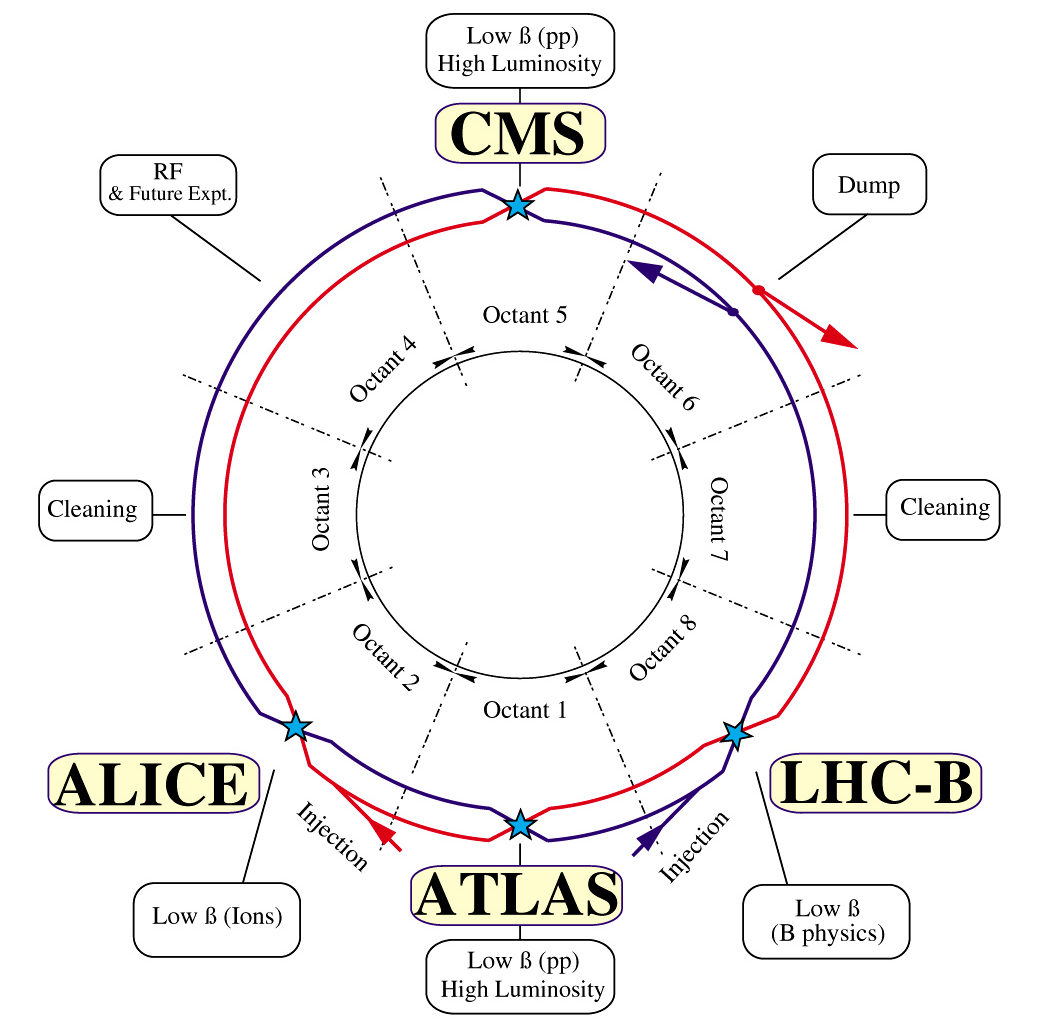
\includegraphics[width=0.95\textwidth]{figures/lhc-pho-1997-060.png}
\caption{A diagram of the LHC with the major experiments labeled \cite{Jean-Luc:841573}.}
\label{fig:lhc-diagram}
\end{center}
\end{figure}

The LHC is designed to accelerate two beams of protons up to energies of 7\TeV each, at instantaneous luminosities up to $10^{34}\percms$. It is also designed to accelerate lead ions up to energies of 1.38\TeV per nucleon, at instantaneous luminosities up to $10^{27}\percms$. The LHC can achieve energies several orders of magnitude higher than LEP in the same tunnel by using protons instead of electrons; the larger mass of protons reduces losses from synchrotron radiation by $(m_{\Pp}/m_{\Pe})^{4} = 1836^{4} = 1.136\times10^{13}$. The use of supercooled superconducting magnets, discussed below, is also crucial. Several stages of CERN accelerators are used to inject proton beams into the LHC, as shown in Fig. \ref{fig:lhc-injectors}. These include the linear accelerator Linac2, the Proton Synchrotron Booster (PSB), the Proton Synchrotron (PS), and the Super Proton Synchrotron (SPS). For lead ions, Linac3 and the Low Energy Ion Ring (LEIR), repurposed from the Low Energy Antiproton Ring (LEAR), are used instead of Linac2 and the PSB, respectively. The accelerated protons are grouped into bunches using radio frequency (RF) electromagnetic fields. The LHC is designed to accommodate a bunch spacing of 25\unit{ns}.

\begin{figure}[hbt]
\begin{center}
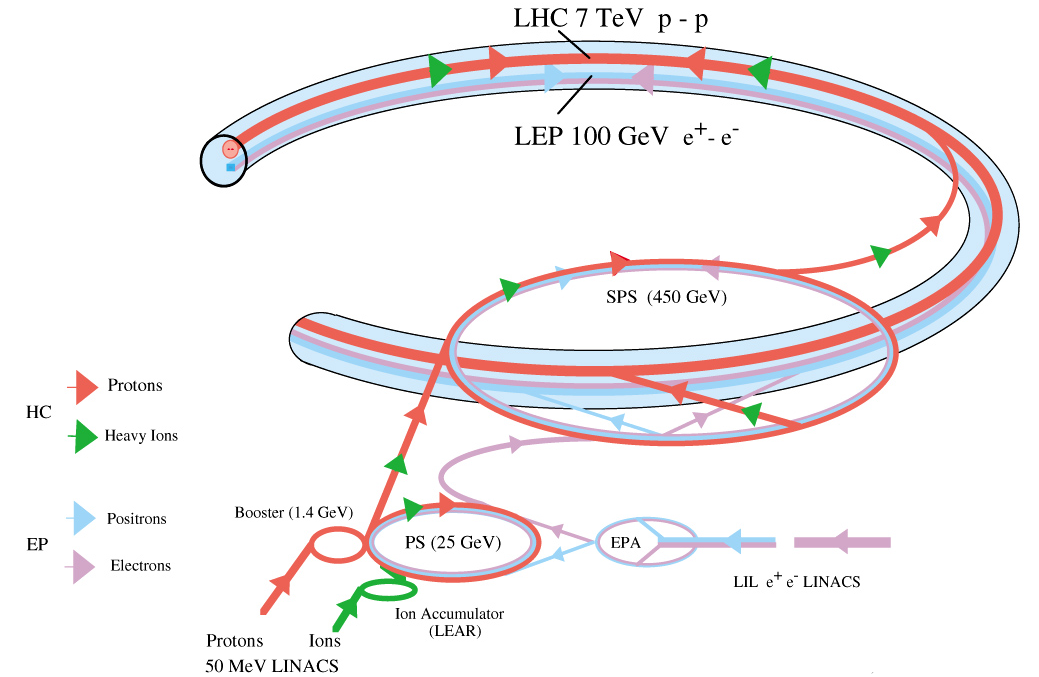
\includegraphics[width=0.95\textwidth]{figures/lhc-pho-1993-008.png}
\caption{A diagram of the CERN accelerators which form the LHC injector \cite{Jean-Luc:841568}.}
\label{fig:lhc-injectors}
\end{center}
\end{figure}

Due to size limitations in the tunnel, the two rings used to accelerate the two proton beams are formed by twin bore magnets. Each magnet has a single mechanical structure and cryostat, in which are placed two coils and two beam channels. The dipole magnet coils use superconducting NbTi Rutherford cables cooled to 1.9\unit{K}, as shown in Fig. \ref{fig:lhc-dipole}, with a design field strength of 8.33\unit{T} for acceleration of protons up to 7\TeV. This extreme cooling is accomplished using superfluid helium. In total, the LHC contains 1232 dipole magnets. Thousands of quadrupole, sextupole, octupole, and decapole magnets are used to correct and focus the beam.

\begin{figure}[hbt]
\begin{center}
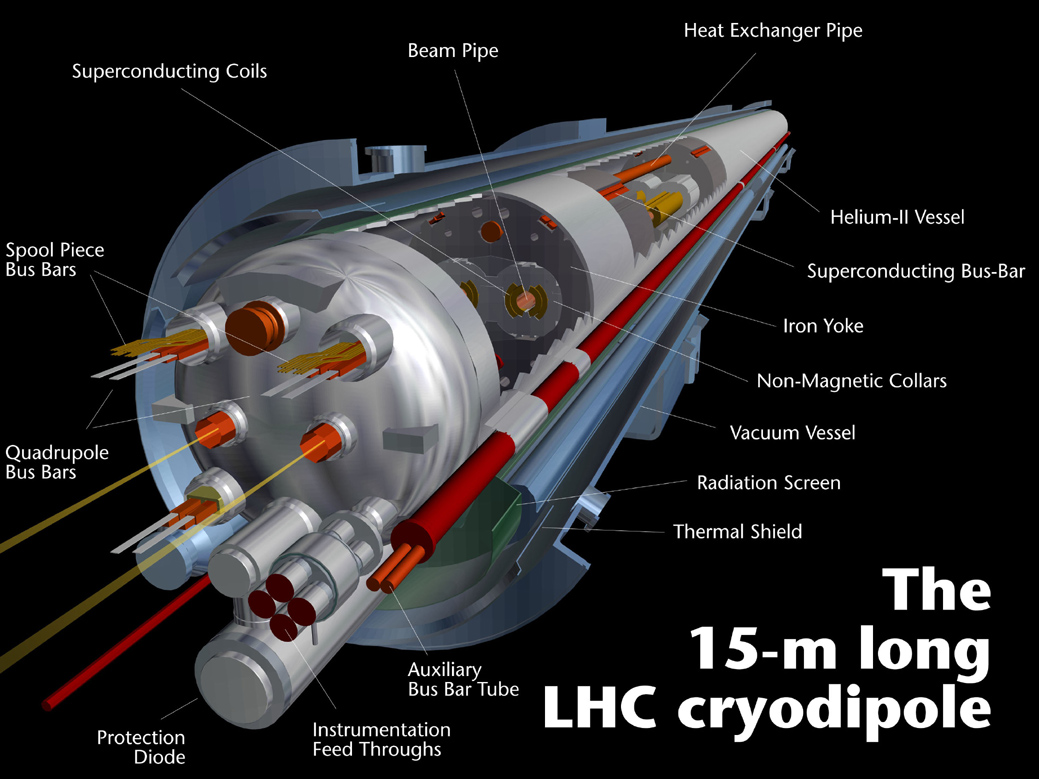
\includegraphics[width=0.95\textwidth]{figures/lhc-pho-1998-299.jpg}
\caption{A diagram of an LHC dipole magnet, with the major components labeled \cite{Dailler:842253}.}
\label{fig:lhc-dipole}
\end{center}
\end{figure}

In 2012, the LHC accelerated proton beams to energies of 4\TeV each, with a peak instantaneous luminosity of $7.67\times10^{33}\percms$ and a bunch spacing of 50\unit{ns}. During that year, it delivered 23.30\fbinv of integrated luminosity to the CMS detector, of which 21.79\fbinv was recorded. In the upcoming 2015 run, the LHC will achieve its design energy, instantaneous luminosity, and bunch spacing.

\section{Tracker}
\label{sec:tracker}

The CMS tracker is the first subdetector to measure charged particles produced in collisions at the IP. It is 5.8\unit{m} long and 2.5\unit{m} in diameter, covering the pseudorapidity range $-2.5 < \eta < 2.5$. Two subsystems make up the tracker: the pixel detector and the silicon strip tracker. The layout of the tracker, with these subsystems labeled, is shown in Fig. \ref{fig:tk-layout}. Due to the tracker's location close to the IP, it experiences severe radiation doses that are expected to range from 0.18 to 84\unit{Mrad} after 500\fbinv of data. Hence, the tracker must be robust against radiation damage, requiring operation at $-10\degC$ and influencing the design of the sensors and electronics. For tracks with momentum of 100\GeV, the tracker has a transverse momentum resolution of 1--2\% for $|\eta|<1.6$; at higher $\eta$, the reduced transverse depth of the tracker degrades the resolution.

\begin{figure}[hbt]
\begin{center}
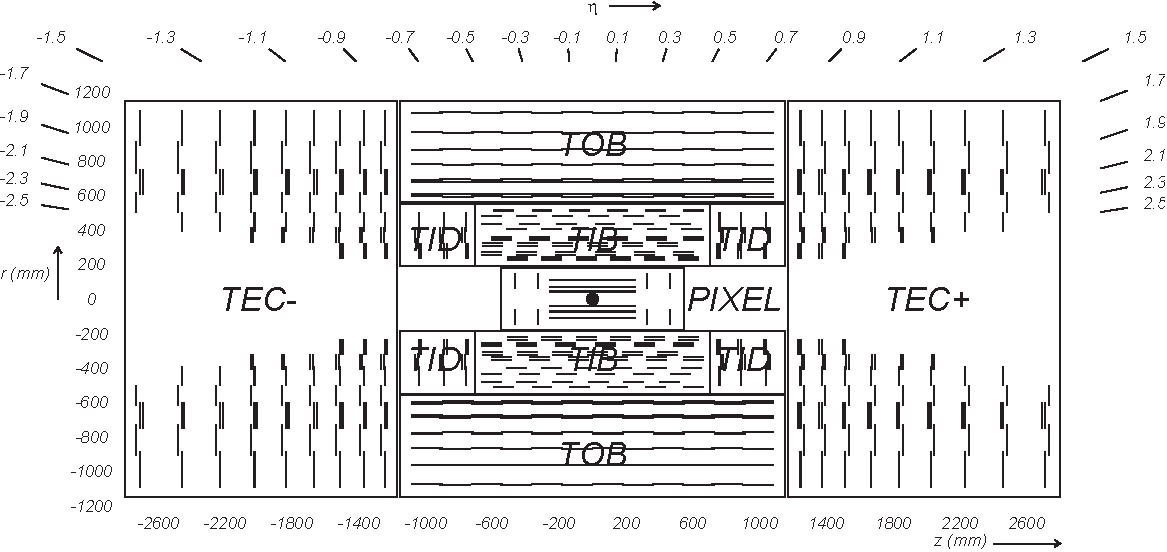
\includegraphics[width=0.95\textwidth]{figures/CMS_tracker.pdf}
\caption{The layout of the CMS tracker, with subsystems labeled.}
\label{fig:tk-layout}
\end{center}
\end{figure}

The pixel detector is the innermost portion of the tracker. It consists of three barrel layers, collectively called BPIX, and two endcap layers, called FPIX. Each pixel cell is a hybrid silicon detector with dimensions $100\times150\mum^{2}$. The small pixel size enables precise track resolutions of 10\mum in the $r$-$\phi$ direction and 20\mum in the $z$ direction. In total, the BPIX comprises 48 million pixels and the FPIX comprises 18 million pixels. The pixel detector is important for many key components of CMS physics analysis. These include the reconstruction of secondary vertices from decays of tau leptons and bottom quarks, as well as producing seed tracks for the strip tracker and the high level trigger.

The silicon strip detector consists of four subsystems. The Tracker Inner Barrel (TIB) has four layers with the three-layer Tracker Inner Disks (TID) at each end; both systems' strips are 320\mum thick. Surrounding the TIB/TID is the Tracker Outer Barrel (TOB), which has six layers. The first four layers of the TOB use 500\mum thick strips, while the last two layers use 122\mum thick strips. The Tracker EndCaps (TEC) have nine disks with up to seven layers of strips, 320\mum thick in the inner four rings and 500\mum thick in the outer three rings. In total, all of these layers contain 9.3 million silicon strips.

The tracker maintained excellent performance during the 2012 run of the LHC. The pixel detector had 97.7\% of channels operational in BPIX and 92.8\% of channels operational in FPIX, while 97.5\% of channels in the strip detector were active. The hit reconstruction efficiencies were greater than 99\% for each layer of the strip detector and greater than 99.5\% for each layer of the pixel except for the first layer of BPIX, which had an efficiency greater than 99.2\% \cite{Veszpremi:2014hpa}. 

\section{Electromagnetic Calorimeter}

The electromagnetic calorimeter (ECAL) is a homogeneous calorimeter constructed entirely of lead tungstate (\pbwo) crystals. The ECAL is divided into two subsystems: the ECAL barrel (EB) and the ECAL endcap (EE). In the endcap region, there is an additional ECAL preshower (ES) detector in front of the EE. Figure \ref{fig:ecal-layout} displays these subsystems. \pbwo has a peak emission wavelength of 425\unit{nm} and many desirable material properties. These properties include high density ($8.28\unit{g/cm}^3$), short radiation length (0.89\cm), short Moli\`{e}re radius (2.2\cm), and fast decay time (6\unit{ns}). The use of homogeneous \pbwo crystals enables precise energy resolution for electromagnetic objects. For photons with $\ET \approx 60\GeV$, the energy resolution ranges from 1.1\% to 2.6\% for the EB and 2.2\% to 5.0\% for the EE. In general, the energy resolution $\sigma$ varies as a function of energy $E$ in \GeVns:
\begin{equation}
\label{eq:ecal-res} \left(\frac{\sigma}{E}\right)^{2} = \left(\frac{S}{\sqrt{E}}\right)^{2} + \left(\frac{N}{E}\right)^{2} + C^{2}.
\end{equation}
In Eq. \eqref{eq:ecal-res}, $S$ is the stochastic term, $N$ is the noise term, and $C$ is the constant term. Typical values for these terms were measured by a test beam to be $S=2.8\%$, $N=12\%$, $C=0.30\%$.

\begin{figure}[hbt]
\begin{center}
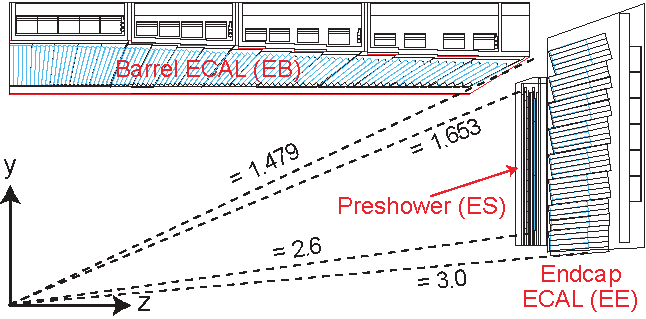
\includegraphics[width=0.95\textwidth]{figures/ECAL_transverse_section.pdf}
\caption{A diagram of the CMS ECAL, with subsystems and $\eta$ ranges labeled.}
\label{fig:ecal-layout}
\end{center}
\end{figure}

The EB contains 61200 \pbwo crystals and covers the range $|\eta|<1.479$. The crystals are arranged in a projective geometry with a tapered shape. The crystal granularity is approximately $0.0174\times0.0174$ in $\eta$-$\phi$, corresponding to dimensions of $22\times22\mm^{2}$ at the front face and $26\times26\mm^{2}$ at the back face. The EB has a depth of 230\mm or 25.8 radiation lengths ($X_{0}$). The scintillation light produced by the \pbwo crystals is read out using avalanche photodiodes (APDs). At 18\degC, the APDs measure approximately 4.5 photoelectrons per \MeVns. The dark current of the APDs is sensitive to radiation exposure. Over the course of the 2012 run, the dark current ranged from 0.3--1.3\muA on average, corresponding to an average noise of 47--57\MeV \cite{CMS:2013ecal}.

The EE contains 14648 \pbwo crystals and covers the range $1.479<|\eta|<3.0$. The crystals are arranged in a non-projective $x$-$y$ geometry, with dimensions of $28.62\times28.62\mm^{2}$ at the front face and $30\times30\mm^{2}$ at the back face. The EE has a depth of 220\mm or 24.7$\,X_{0}$. Vacuum phototriodes (VPTs) are used as the photodetectors to read out the scintillation light from the \pbwo crystals. They collect approximately 4.5 photoelectrons per \MeVns at 18\degC. During the 2012 run, the average noise ranged from 180--220\MeV, with a more dramatic increase up to 600\MeV at high $\eta$ because of the high radiation dose \cite{CMS:2013ecal}.

The ES is intended to identify neutral pions in the endcap region, covering the range $1.653<|\eta|<2.6$. It is a sampling calorimeter with two layers of lead absorber and silicon strip detectors. The first layer of lead absorber has a thickness of 2$\,X_{0}$, while the second layer has a thickness of 1$\,X_{0}$. Each layer of silicon strips is 320\mum thick and can collect 3.6\unit{fC} of charge from a minimum ionizing particle.

%add percentage of live channels for EB and EE in 2012 run? and HE raddam?

\section{Hadron Calorimeter}

The hadron calorimeter (HCAL) is a sampling calorimeter which measures the energy of hadronic particles. The HCAL is especially important for measuring neutral hadrons, which do not leave tracks in the tracker. In addition, by containing all hadronic activity in each event within $|n|<5$, the HCAL enables the measurement of \met caused by neutrinos and other theoretical weakly-interacting particles. The HCAL consists of four subsystems. Three of these subsystems use similar technology: the HCAL barrel (HB), the HCAL endcap (HE), and the HCAL outer (HO). The fourth subsystem, the HCAL forward (HF), uses an alternative technology necessary to survive the high radiation doses at its forward location. The locations of the various HCAL subsystems in the CMS detector are shown in Fig. \ref{fig:hcal-layout}. The calorimeter system, combining the ECAL and the HCAL, can measure jets with a resolution $\sigma/E \approx 100\% / \sqrt{E\,[\GeVns]} \oplus 5\%$ that varies with the jet energy $E$.

\begin{figure}[hbt]
\begin{center}
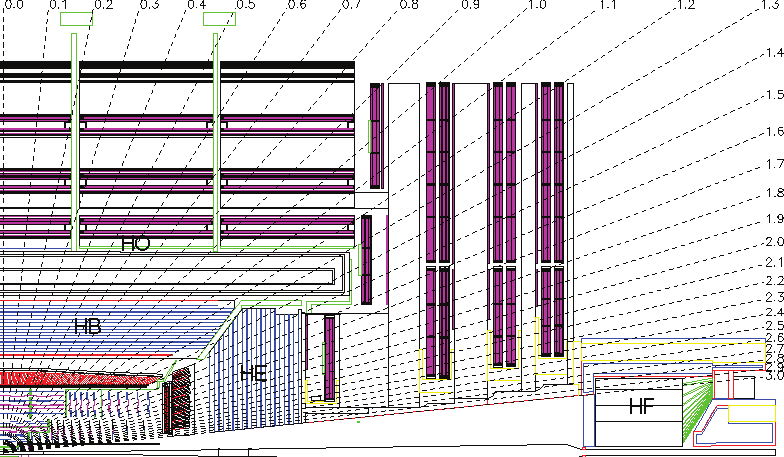
\includegraphics[width=0.95\textwidth]{figures/HCAL_subdet.pdf}
\caption{The layout of the HCAL subsystems HB, HE, HO, and HF in the CMS detector.}
\label{fig:hcal-layout}
\end{center}
\end{figure}

The HB is a 16-layer sampling calorimeter covering the range $|\eta|<1.3$. The absorbing layers are made of C26000 cartridge brass, composed of 70\% copper and 30\% zinc. Cartridge brass has a density of $8.53\unit{g/cm}^3$, a radiation length of 1.49\cm, and a nuclear interaction length of 16.42\cm. The first absorbing layer in the HB is a 40-mm-thick steel plate. The next eight absorbing layers are 50.5-mm-thick brass plates, and the subsequent six absorbing layers are 56.5-mm-thick brass plates. The last absorbing layer is a 75-mm-thick steel plate. The overall thickness of the HB absorber ranges from 5.82$\,\lambda_{0}$ at $\eta=0$ to 10.6$\,\lambda_{0}$ at $|\eta|=1.3$. The EB in front of the HB has a thickness of 1.1$\,\lambda_{0}$ and can measure the electromagnetic portions of early developing hadronic showers. The scintillating layers consist of 3.7-mm-thick Kuraray SCSN81 plastic scintillator, a polystyrene base doped with fluors. The exception is Layer 16, which has a thickness of 9\mm, in order to sample more from late developing hadronic showers. At the front of the HB, before the first absorbing layer, is the scintillator Layer 0, which is 9\mm of Bicron BC408 plastic scintillator, a polyvinyltoluene base doped with fluors. Layer 0 samples the energy deposited by hadronic showers in the dead material between the EB and the HB. The scintillator tiles are arranged in a projective geometry with a granularity of $0.087\times0.087$ in $\eta$-$\phi$. In total, the HB has 16 $\eta$ divisions called towers, 36 $\phi$ divisions, and approximately 70000 tiles. The light from the scintillators is collected by Kuraray Y-11 green wavelength shifting (WLS) fiber, which is placed in a $\sigma$-shaped groove in the scintillator tiles. The wavelength-shifted light from multiple layers is brought together and read out by hybrid photodiodes (HPDs). These photodetectors were chosen because of their large dynamical range and low sensitivity to magnetic fields.

The thinness of the HB at low $\eta$ prevents it from fully containing hadronic showers, so the HO is added to act as an extension of the calorimeter system. The HO uses the same scintillator tile technology as the HB: 3.7-mm-thick SCSN81 with Y-11 WLS fiber and granularity $0.087\times0.087$ in $\eta$-$\phi$, read out by HPDs. The HO is divided into five rings, each with a width of 2.536\unit{m} in the $z$ direction, based on the structure of the iron return yoke outside of the solenoid. In the central Ring 0, the HO has two scintillating layers, one inside the solenoid and one outside of it. In the other rings, the HO has one scintillating layer outside of the solenoid. The thickness of the absorbing iron layer formed by the solenoid is 19.5\cm, extending the total depth of the calorimeter system to a minimum of 11.8$\,\lambda_{0}$.

The HE is a 17-layer sampling calorimeter covering the range $1.3<|\eta|<3.0$. Each absorbing layer consists of 79-mm-thick cartridge brass, the same material used for the HB absorbing layers. The scintillating layers use the same technology as the HB and the HO. In total, the HE contains 20916 scintillator tiles. The granularity of the tiles is the same as HB for $|eta|<1.6$; for higher $\eta$, they become coarser at approximately $0.17\times0.17$ in $\eta$-$\phi$. Unlike the HB, the scintillating layers in each tower are split into multiple groups called depths before being read out by HPDs. A diagram of the depth segmentation scheme is shown in Fig. \ref{fig:hcal-depths}. This depth segmentation allows for more precise recalibration of the HE, which experiences a higher radiation dose than the HB. Towers 27, 28, and 29, which are the closest to the beamline, have three readout depths, while the other towers have two readout depths. The crossover region between the HB and the HE, towers 15 and 16, also utilize depth segmentation. As in the HB, Layer 0 in the HE consists of 9-mm-thick BC408 to sample from the dead material between the EE and the HE. The combined calorimeter system, including both the EE and the HE, has an approximate thickness of 10$\,\lambda_{0}$.

The HF covers the range $3.0<|\eta|<5.0$, with no ECAL in front of it. It consists of a steel absorber structure with a thickness of 165\cm or 10$\,\lambda_{0}$. Polymer-cladded quartz fibers with diameter 800\mum are embedded in the steel absorber. The fibers are bundled together to form 13 towers in a non-projective $x$-$y$ geometry with granularity $0.175\times0.175$ in $\eta$-$\phi$. Over 1000\unit{km} of fiber is used in the HF. Half of the fibers run for the full 165\cm depth of the detector, while the other half start 22\cm into the detector. Each type of fiber is read out separately in order to distinguish electromagnetic showers from hadronic showers. The fibers measure particle showers using Cherenkov light, which is read out by photomultiplier tubes (PMTs). They measure approximately 1 photoelectron for every 4\GeV of energy deposited. This alternative design was necessary to ensure the radiation hardness of the HF, parts of which can experience 100\unit{Mrad/year}.

\begin{figure}[hbt]
\begin{center}
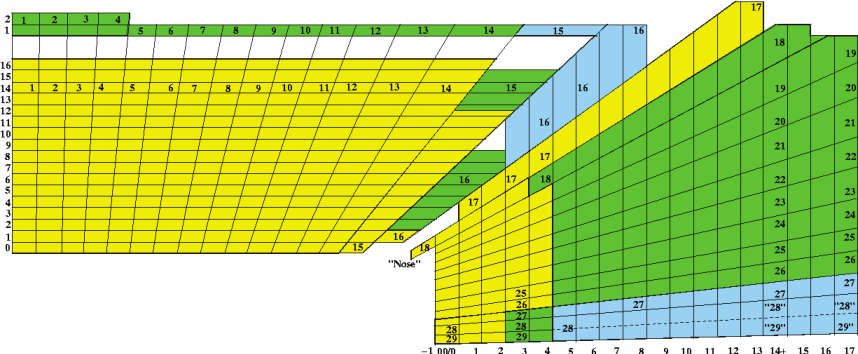
\includegraphics[width=0.95\textwidth]{figures/HCAL_tower_segmentation.pdf}
\caption{A diagram of the depth segmentation scheme in the HB and the HE.}
\label{fig:hcal-depths}
\end{center}
\end{figure}

%add percentage of live channels for HCAL in 2012 run?

\section{Solenoid}

The superconducting solenoid is the central feature of the CMS detector. The solenoid provides a magnetic field of 3.8\unit{T} within the volume formed by its diameter of 6\unit{m} and length of 12.5\unit{m}. This strong magnet field is necessary so that high energy charged particles bend sufficiently for the tracker to measure their momenta accurately. At full current, the solenoid has a stored energy of 2.35\unit{GJ}. The magnet is constructed from a 4-layer winding of reinforced NbTi conductor, cooled to 4.5\unit{K}. It is split into five rings of equal length. The cold mass of the magnet is 220 tons, and the high ratio between the stored energy and the cold mass, 11.6\unit{KJ/kg}, causes a significant mechanical deformation of 0.15\% when the magnet is powered. Figure \ref{fig:solenoid} shows an artistic rendering of the solenoid.

\begin{figure}[hbt]
\begin{center}
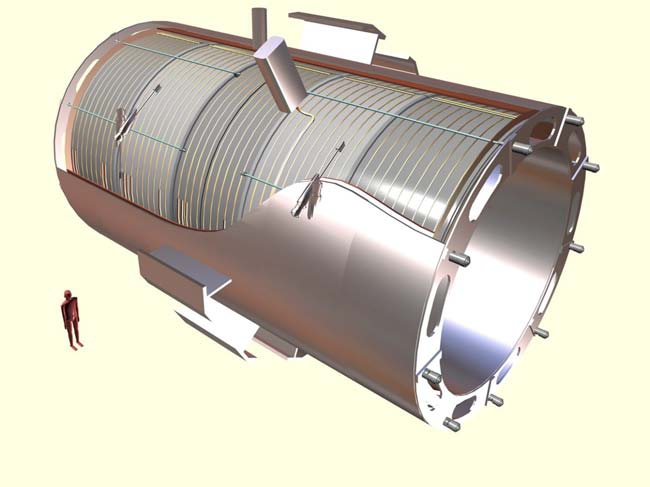
\includegraphics[width=0.95\textwidth]{figures/CMS_solenoid.jpg}
\caption{An artistic rendering of the CMS solenoid, showing the five rings placed inside the cryostat, along with the support structure.}
\label{fig:solenoid}
\end{center}
\end{figure}

\section{Muon System}
\label{sec:muon-system}

The identification and measurement of muons is a major focus of the CMS experiment. The CMS muon system comprises three subsystems, each utilizing different gaseous particle detection technology. In the barrel region, drift tubes (DTs) are used. In the endcap region, cathode strip chambers (CSCs) are used. Resistive plate chambers (RPCs) are also used in both regions. The muon systems are built into the iron yoke, which consists of five barrel rings and six endcap disks weighing 10000 tons in total. The yoke confines the outer magnetic field from the return flux from the solenoid and absorbs stray hadrons. The layout of the muon system is shown in Fig. \ref{fig:muon-system}. The momentum resolution of the muon system by itself is approximately 9\% for $\pt<200\GeV$ with low $\eta$ and low $p$. For 1\TeV muons, the resolution varies between 15\% and 40\%, depending on $|\eta|$. When the muon system measurements are combined with measurements from the tracker, the 1\TeV muon resolution is improved to 5\%.

\begin{figure}[hbt]
\begin{center}
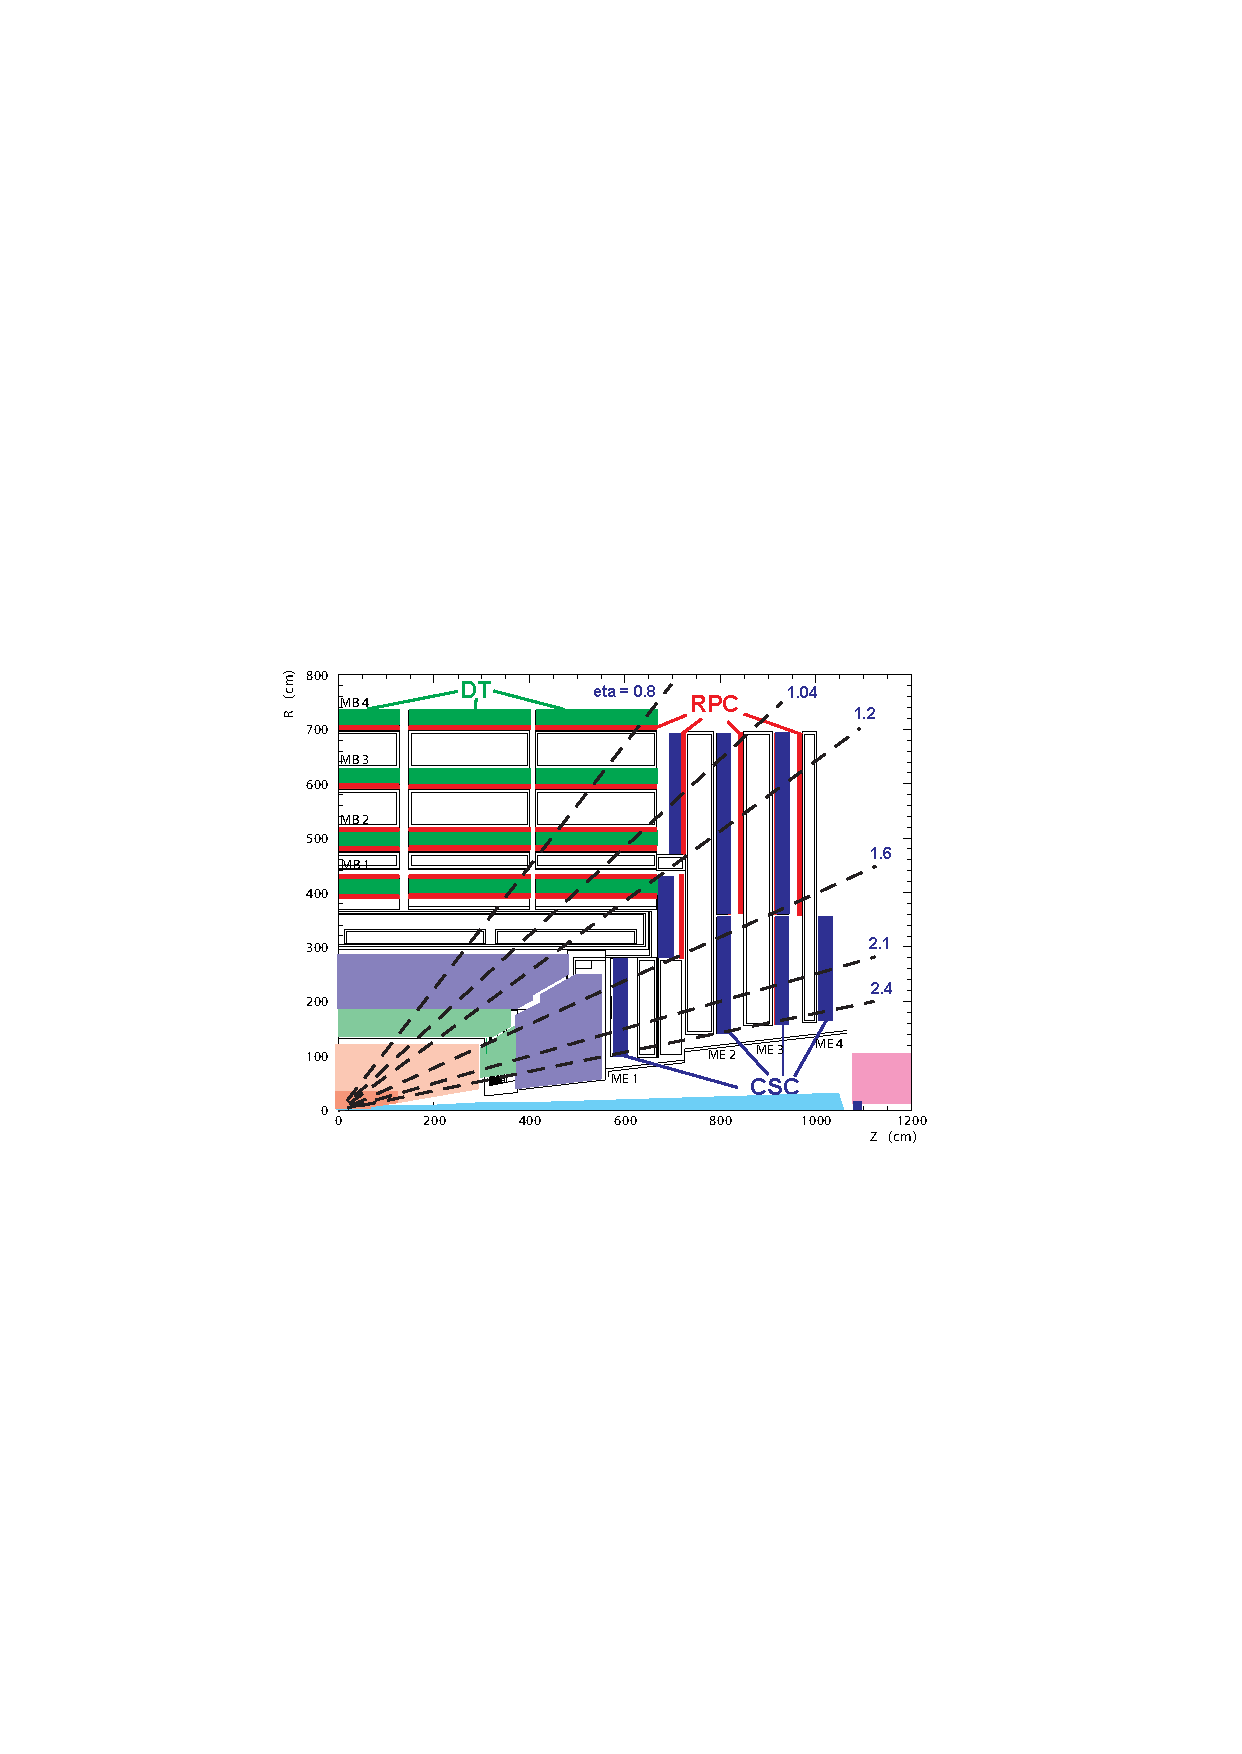
\includegraphics[width=0.95\textwidth]{figures/CMS_muon_system.pdf}
\caption{The layout of the muon system, with the three subsystems labeled.}
\label{fig:muon-system}
\end{center}
\end{figure}

The DTs are divided into four stations, which together cover the range $|\eta|<1.2$ and are labeled MB1 through MB4 (Muon Barrel). The first three stations each contain twelve chambers divided into three groups of four. Two of the groups of four measure the $r$-$\phi$ coordinate of muons, while the third group of four measures the $z$ coordinate. MB4 does not include a group of chambers that measures $z$. All four stations together contain 250 DTs with a total of 172000 sensitive wires. The gas used in the DTs is a mixture of 85\% Ar and 15\% $\text{CO}_2$, and the anode wires are gold-plated stainless steel with a diameter of 50\mum. Within $|\eta|<0.8$, the MB stations alone can reconstruct high-\pt muon tracks with an efficiency exceeding 95\%. The global $r$-$\phi$ resolution is 100\mum.

The CSCs are also divided into four stations and cover the range $0.9<|\eta|<2.4$. The four stations are labeled ME1 through ME4 (Muon Endcap). Each station is divided into several groups as follows: ME1 has three groups of 72 CSCs; ME2 and ME3 each have one group of 36 CSCs and another group of 72 CSCs; ME4 has one group of 36 CSCs. The total number of CSCs is thus 468. The cathode strips are arranged in the radial direction to measure the $r$-$\phi$ coordinate, while the anode wires are perpendicular to the strips to measure $\eta$. There are approximately 220000 cathode strip readout channels and 180000 anode wire readout channels. The CSC gas mixture is set at 40\% AR, 50\% $\text{CO}_2$, and 10\% $\text{CF}_4$. The cathode strips are formed from a fiberglass/epoxy material called FR4, coated with 36-$\mu$m-thick copper. The anode wires are made of gold-plated tungsten with a diameter of 50\mum. The first group of ME1 CSCs uses slightly thinner wire with 30\mum diameter and has some other slightly modified properties.

To complement the DTs and CSCs, RPCs are installed in both the barrel and endcap regions, covering the range $|\eta|<1.6$. The RPCs are primarily used to provide muon trigger information, due to fast tagging capabilities which allow them to precisely identify the bunch crossing time of muon candidate events. MB1 and MB2 each have one internal and one external group of RPCs, relative to the DTs; MB3 and MB4 each have two internal groups of RPCs. These groups together comprise 480 chambers. In the endcap, there are three RPC stations mounted in concentric circles on the iron yoke disks, with a total of 144 chambers. The RPCs are parallel plate detectors filled with a gas mixture of 96.2\% $\text{C}_2\text{H}_2\text{F}_4$, 3.5\% $i\text{C}_4\text{H}_{10}$, and 0.3\% $\text{SF}_6$.

%add percentage of live channels for muon system in 2012 run?

\section{Trigger}

The CMS trigger is necessary to reduce the roughly 1\unit{MHz} rate of collision events produced by the LHC to a rate which can be stored and processed. The trigger system consists of two stages. The first stage uses hardware and is called the Level-1 (L1) Trigger. The L1 Trigger is designed to have a maximum output rate of 100\unit{kHz}. The second stage is the High Level Trigger (HLT), which uses software and reduces the output rate to $\mathcal{O}(100\unit{Hz})$.

The L1 Trigger uses custom-built programmable electronics, including field-programmable gate arrays (FPGAs), application-specific integrated circuits (ASICs), and memory lookup tables (LUTs). All of the subdetectors send input to the L1 Trigger, which is organized into local, regional, and global components as shown in Fig. \ref{fig:L1-trigger}. The local components, Trigger Primitive Generators (TPGs), are constructed from energy deposits in the calorimeters and track segments or hit patters from the muon system.

The TPGs from the ECAL, the HCAL, and the HF are combined into the Regional Calorimeter Trigger (RCT). The RCT groups calorimeter trigger towers into regions, which are made up of four towers in the barrel and endcap, and one tower in the HF. These regions are used to determine electron and photon candidates, as well as transverse energy sums (\sumet) and tau-jet vetoes. The RCT also passes MIP and isolation information to the muon triggers. Using information from the RCT, the Global Calorimeter Trigger (GCT) determines jet candidates and counts, providing up to four jets and four tau-jets from the central HCAL and four jets from the HF. The GCT also determines total \ET, \met, and \HT, which is calculated as \sumet for all jets above a certain threshold.

In parallel, the muon DT, CSC, and RPC systems each produce their own local triggers. The Regional Muon Trigger (RMT) contains the DT and CSC Track Finders (DTTF, CSCTF) which make tracks using segments from their respective subdetectors. As mentioned in Sec. \ref{sec:muon-system}, the RPCs act as a dedicated trigger using their timing resolution of 1\unit{ns} to determine bunch crossing times. The Global Muon Trigger (GMT) combines the information from the RMT and RPCs to produce up to four muon candidates in each of the barrel and endcap regions. These candidates include the following information: \pt, charge, $\eta$, $\phi$, a quality code, MIP, and isolation.

Finally, the Global Trigger (GT) combines the GCT and GMT candidates and quantities to decide whether or not to keep the event, based on a set of L1 triggers with different criteria. The GT also uses information from the Trigger Control System (TCS) regarding the status of the subdetector readout and data acquisition systems. The Timing, Trigger, and Control (TTC) system is used to return the GT decision, called the Level-1 Accept (L1A), to the various subdetectors. This entire process is completed within 3.2\mus.

\begin{figure}[hbt]
\begin{center}
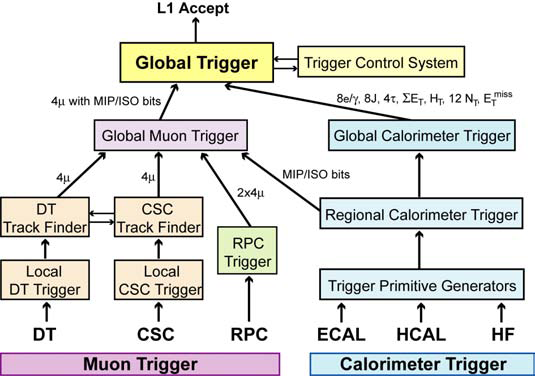
\includegraphics[width=0.95\textwidth]{figures/L1_architecture.png}
\caption{The architecture of the L1 Trigger.}
\label{fig:L1-trigger}
\end{center}
\end{figure}

The HLT further analyzes events which pass the L1A decision. Using a farm of roughly 1000 commercial processors comprised of over 13000 central processing units (CPUs), it approximately emulates the full offline reconstruction algorithms described in Ch. \ref{ch:reconstruction}. Like the L1 Trigger, the HLT uses a set of triggers with different criteria, called the trigger menu. Different trigger menus are constructed for various conditions, including different instantaneous luminosity levels and different types of collisions or measurements. The selected menu can be changed during the operation of the detector in response to new conditions. Events which pass the HLT decision are sorted into primary datasets (PDs) with minimal overlap. The HLT output includes several streams, including monitoring and calibration streams in addition to the primary stream of physics events.

During the 2012 run, the L1 Trigger operated at rates up to 100\unit{kHz} with only 3\% dead time \cite{Brooke:2013hnf}. The HLT operated at rates up to 1\unit{kHz} and took an average of 200\unit{ms} to process an event \cite{Trocino:2014jya}. This processing speed is two orders of magnitude faster than the full offline reconstruction. Around 600\unit{Hz} of HLT output data was ``parked'', or recorded to disk in a raw format before being processed. This data parking scheme took advantage of the impending 2013-2014 long shutdown for collider and detector upgrades, when CPUs would be available to process the extra data. The parked data was collected using alternative trigger menus designed to enable precision measurements and new physics searches in unexplored kinematic regions. CMS also engaged in ``data scouting'', performing simple analyses on partially-reconstructed events, for example keeping only HLT-reconstructed jets, from processes which would normally have rates too high to be accepted by the trigger. These simple analyses searched for noticeable deviations from SM predictions in order to indicate possible advantageous changes to the trigger menus.

\section{Luminosity Measurement}

The fine resolution of the CMS pixel detector (Sec. \ref{sec:tracker}) implies that a given pixel will tend to be activated by one track at most per bunch crossing. A minimum bias interaction creates an average of 200 clusters, with each cluster containing an average of 5 pixels \cite{CMS-PAS-LUM-12-001}. Even with 100 pileup events per bunch crossing, the pixel detector will have an occupancy as low as 0.1\%. The number of pixel hits should thus scale linearly with the number of interactions per bunch crossing for instantaneous luminosities up to and even beyond the LHC design performance. Equation \eqref{eq:pixel-lumi} shows how the instantaneous luminosity $\mathcal{L}$ is related to the average number of pixel clusters per event $\langle n \rangle$ \cite{CMS-PAS-LUM-13-001}:
\begin{equation} \label{eq:pixel-lumi}
\mathcal{L} = \frac{\nu \langle n \rangle}{\sigma_\text{vis}}.
\end{equation}
Here, $\nu = 11246\unit{Hz}$ is the LHC revolution frequency, $\langle n \rangle$ is defined as $\mu n_{1}$ where $\mu$ is the number of collisions per bunch crossing and $n_{1}$ is the average number of clusters per collision, and the visible cross section $\sigma_\text{vis}$ is defined as $\sigma_\text{T} n_{1}$ where $\sigma_\text{T}$ is the total inelastic cross section. A Van der Meer scan is used to calibrate $\sigma_\text{vis}$. In 2012, CMS measured the total integrated luminosity with a systematic uncertainty of 2.6\% using this method.

The HF is used as a second method of measuring the luminosity. This is possible because the HF can be run safely during unstable beams \cite{CMS-PAS-LUM-13-001}. Information from the HF can be used to measure the luminosity in two different ways. The average fraction of empty towers can be related to the mean number of interactions per crossing, or the average transverse energy per tower can be linearly related to the luminosity. It can make an online determination of the average luminosity to a statistical uncertainty of 1\% in under 1\unit{s}. However, the calibration of this measurement can drift over long time periods due to changes in the gain of the HF PMTs. In practice, the increase in pileup interactions observed during the 2012 run moves the HF response into a nonlinear regime, limiting the accuracy of this method. Because of these limitations, the HF method is utilized primarily as a cross-check for the pixel cluster counting method.